%\begin{figure*}
%	\centering
%	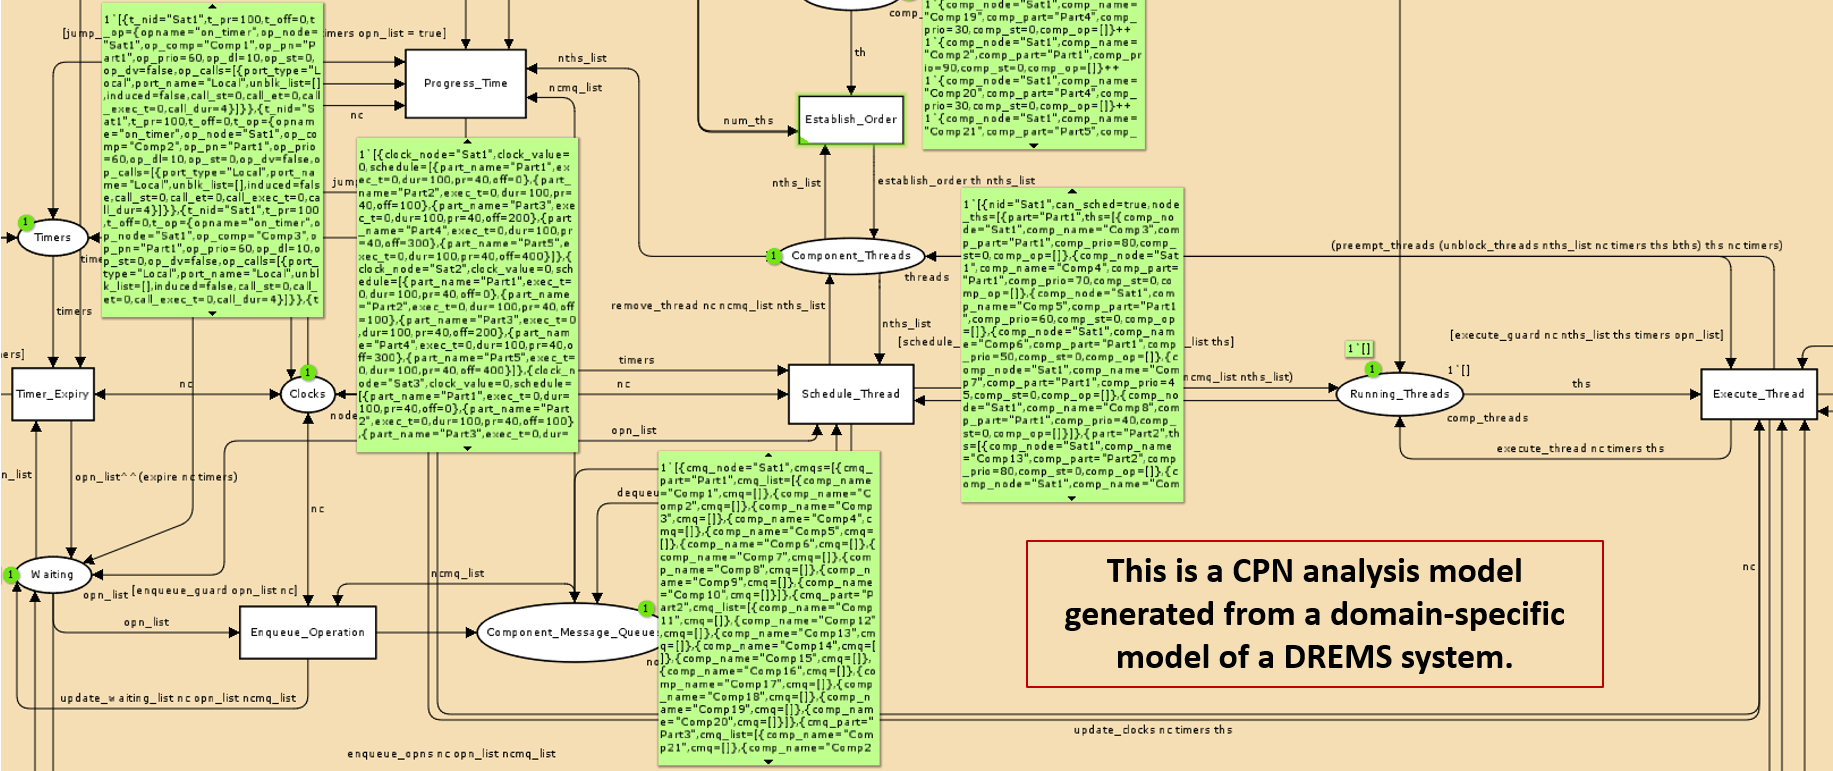
\includegraphics[width=5.8in]{./figs/Generated_Model}
%	\caption{Generated Analysis Model}
%\end{figure*}

\section{Modeling Temporal Behavior}
\label{sec:Modeling}

%\subsection{Modeling Component Business Logic}

The execution of component operations service the various periodic or aperiodic interaction requests coming from either a timer or other connected (possibly distributed) components. Each operation is written by an application developer as a sequence of execution \emph{steps}. Each step could execute a unique set of activities, e.g. perform a local calculation or a library call, initiate an interaction with another component, process a response from external entities, and it can have data-dependent, possibly looping control flow, etc. The behavior derived by the combination of these steps contribute to the worst-case execution of the component operation. The behavior may include non-deterministic delays due to component interactions while being constrained by the  temporally partitioned scheduling scheme and hardware resources. This section briefly describes the various aspects of this behavior specification that are general enough to be applicable to a range of component-based systems.

\begin{figure}[ht]
	\centering
	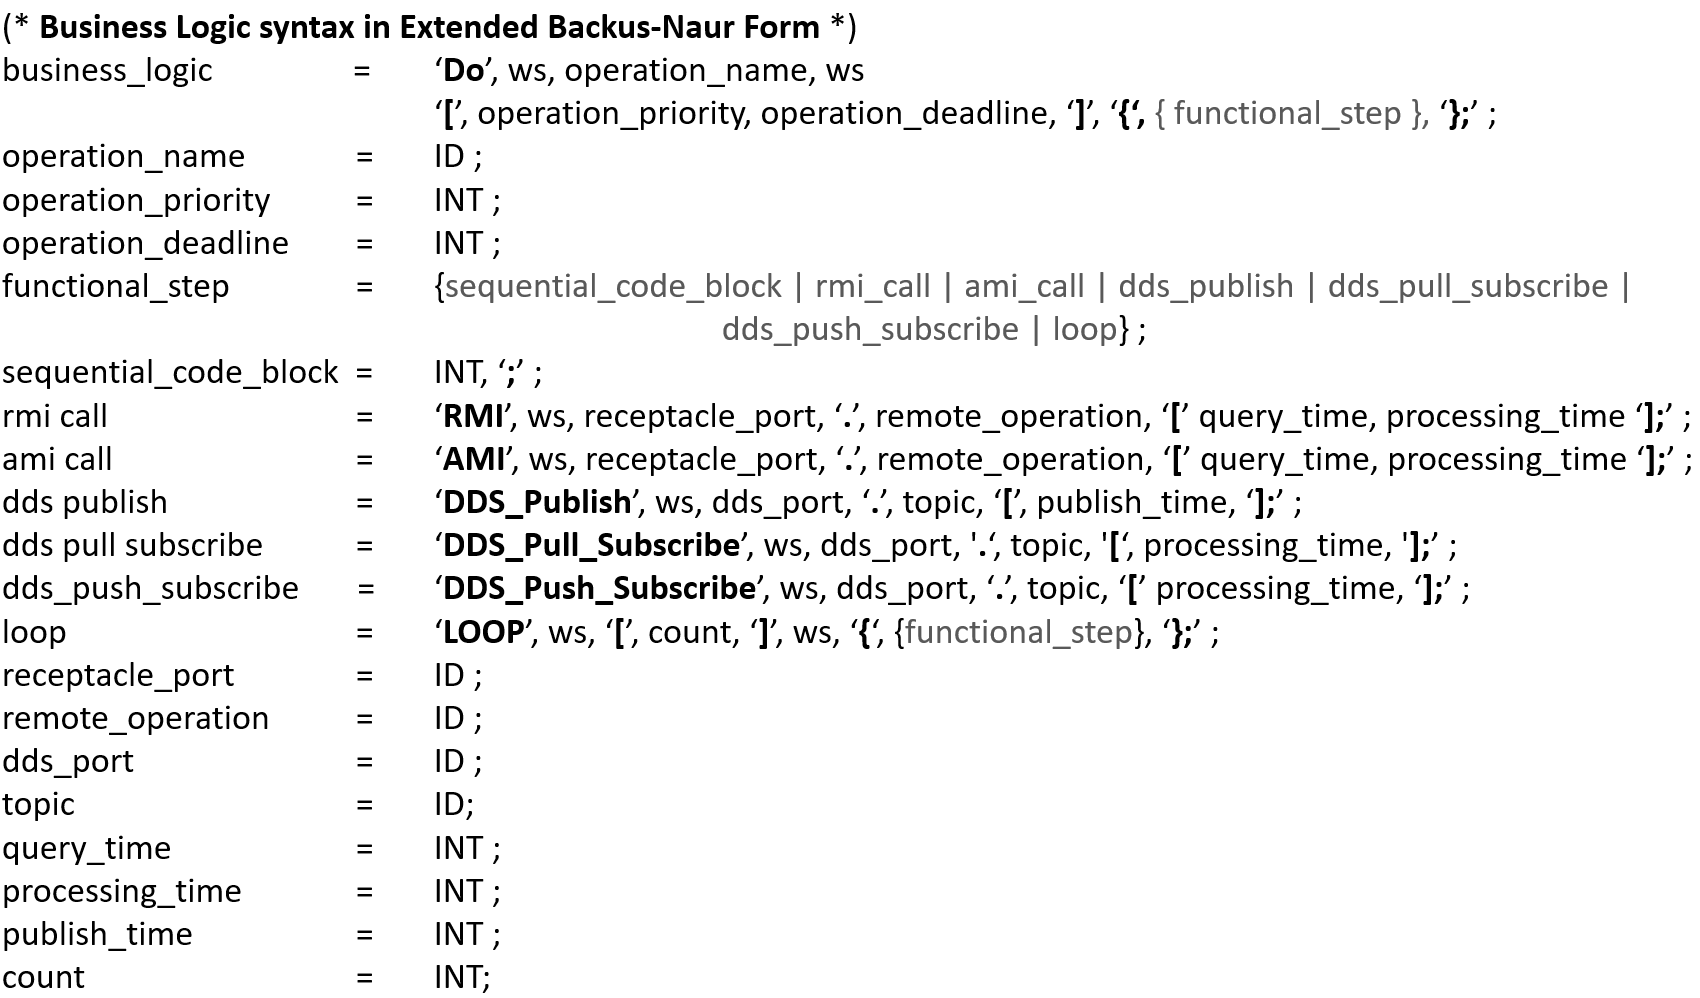
\includegraphics[width=0.5\textwidth]{./figs/BL-EBNF}
	\caption{Modeling the Business Logic of Component Operations}
	\label{fig:ebnf}
\end{figure}

Figure \ref{fig:ebnf} shows the Extended Backus-Naur form representation of the grammar used for modeling the business logic of component operations. The symbol \emph{ID} represents identifiers, a unique grouping of alphanumeric characters, and the symbol \emph{INT} represents positive integers. Each operation is characterized by a unique name, a priority, and a deadline. The priority is an integer used to resolve scheduling conflicts between operations \emph{provided} by the same component when multiple messages from other entities are received. The arbitration is handled by the component-level scheduler. The deadline of the operation is the worst-case time that can elapse after the operation is marked as \emph{ready} and the completion of the operation. The business logic of every component operation is modeled as a sequence of steps, each with an assigned worst-case execution time. We broadly classify these steps into (1) blocks of sequential code, (2) peer-to-peer synchronous and asynchronous remote calls, (3) anonymous publish/subscribe distribution service calls, (4) blocking and non-blocking I/O interactions and (5) bounded control loops. 

Notice the integration of timing properties such as worst-case function call times (\emph{query\_time}), worst-case argument processing times (\emph{processing\_time}) and DDS publish times (\emph{publish\_time}). If these expected delays are set to zero, the analysis will execute these interactions in a single synchronous step taking no time. However, in reality these steps still take a non-zero amount of time to execute. Therefore, if such metrics are not known then these values can be set to zero and an overall worst-case execution time can be set per operation. This is the maximum amount of time that can elapse after the component operation has begun to execute. This time will include all component interactions and network delays that affect the operation's execution.